\documentclass[aspectratio=169,11pt]{beamer}
\usepackage[T1]{fontenc}
\usepackage{lmodern,amsmath,amssymb,mathtools,bm,booktabs,array,graphicx,tikz}
\usetikzlibrary{arrows.meta,positioning,calc,decorations.pathreplacing,patterns}
\definecolor{ink}{HTML}{17344D}\definecolor{accent}{HTML}{087E8B}\definecolor{pale}{HTML}{EDF5F5}\definecolor{gold}{HTML}{AD6B19}
\providecommand{\dd}{\,\mathrm{d}}\providecommand{\R}{\mathbb{R}}
\providecommand{\E}{\mathbb{E}}\providecommand{\Var}{\operatorname{Var}}
\providecommand{\Cov}{\operatorname{Cov}}\providecommand{\diag}{\operatorname{diag}}
\providecommand{\norm}[1]{\left\lVert#1\right\rVert}
\providecommand{\abs}[1]{\left|#1\right|}
\usefonttheme{professionalfonts}
\setbeamercolor{normal text}{fg=black,bg=white}
\setbeamercolor{frametitle}{fg=ink,bg=white}
\setbeamercolor{title}{fg=ink}\setbeamercolor{structure}{fg=accent}
\setbeamercolor{block title}{fg=ink,bg=pale}\setbeamercolor{block body}{fg=black,bg=pale!40}
\setbeamercolor{alerted text}{fg=accent}
\setbeamerfont{frametitle}{size=\Large,series=\bfseries}
\setbeamerfont{title}{size=\LARGE,series=\bfseries}
\setbeamertemplate{navigation symbols}{}
\setbeamersize{text margin left=.7cm,text margin right=.7cm}
\setbeamertemplate{frametitle}{\vspace{.18cm}\insertframetitle\par\vspace{.1cm}{\color{accent}\hrule height .6pt}\vspace{.12cm}}
\newcommand{\notestarget}{notes.pdf}\newcommand{\noteslabel}{Notes}
\setbeamertemplate{footline}{\hspace{.7cm}\color{ink}\scriptsize Computational Cardiology\quad\href{\notestarget}{\noteslabel}\hfill\insertframenumber\,/\,\inserttotalframenumber\hspace{.7cm}\vspace{.18cm}}
\setbeamercovered{invisible}
\hypersetup{pdfauthor={Zan Ahmad},pdftitle={Shape comparisons, deformation penalties and geometric matching},pdfpagemode=UseNone}
\begin{document}
\begin{frame}[plain]\vfill
{\small\color{accent} Computational Cardiology \quad Lecture 14}\par\medskip
{\raggedright\hyphenpenalty=10000\exhyphenpenalty=10000\LARGE\bfseries\color{ink} Shape comparisons, deformation penalties and geometric matching}\par\bigskip
Zan Ahmad\par\smallskip
{\small Fall 2024}\par\vfill\end{frame}
\renewcommand{\notestarget}{notes.pdf\#note-a-finite-cohort-and-its-comparison-rule}
\begin{frame}[t,fragile,label=slide-a-comparison-requires-an-invariance-choice]{A comparison requires an invariance choice}
Raw coordinate RMS includes pose, cyclic start and shape.\pause{} We remove proper rigid motion and cyclic start while retaining physical scale and traversal direction.
\end{frame}
\renewcommand{\notestarget}{notes.pdf\#note-a-finite-cohort-and-its-comparison-rule}
\begin{frame}[t,fragile,label=slide-a-known-finite-cohort]{A known finite cohort}
A is the reference; B is a rigid copy; C is $15\%$ larger; D has a local displacement; E has a shifted starting index.\pause{} These relationships are constructed, not discovered.
\end{frame}
\renewcommand{\notestarget}{notes.pdf\#note-cyclic-rigid-alignment}
\begin{frame}[t,fragile,label=slide-cyclic-rigid-discrepancy]{Cyclic rigid discrepancy}
\[d_{rc}(X,Y)=\min_{k,R,t}\left(\frac1n\sum_j\|x_j-(y_{j+k}R+t)\|^2\right)^{1/2}.\]\pause{} $R\in SO(2)$ and indices wrap modulo $n$.
\end{frame}
\renewcommand{\notestarget}{notes.pdf\#note-cyclic-rigid-alignment}
\begin{frame}[label=slide-enumerate-the-starting-index-panel-1]{Raw index RMS}
\centering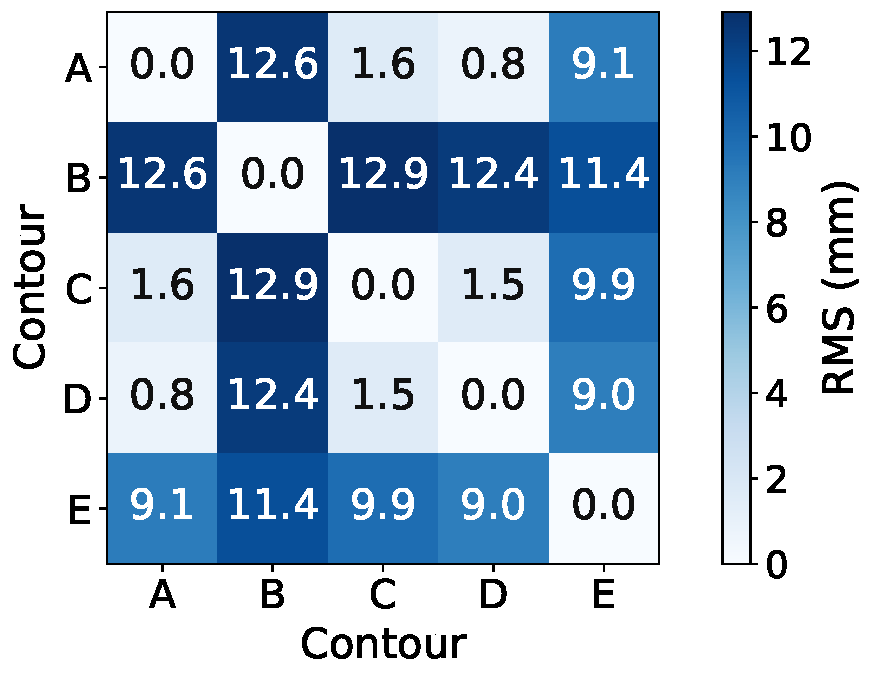
\includegraphics[width=.98\linewidth,height=.69\textheight,keepaspectratio]{presentation-figures/cohort-distances-panel-1.pdf}\end{frame}
\renewcommand{\notestarget}{notes.pdf\#note-cyclic-rigid-alignment}
\begin{frame}[label=slide-enumerate-the-starting-index-panel-2]{Rigid +\allowbreak{} cyclic RMS}
\centering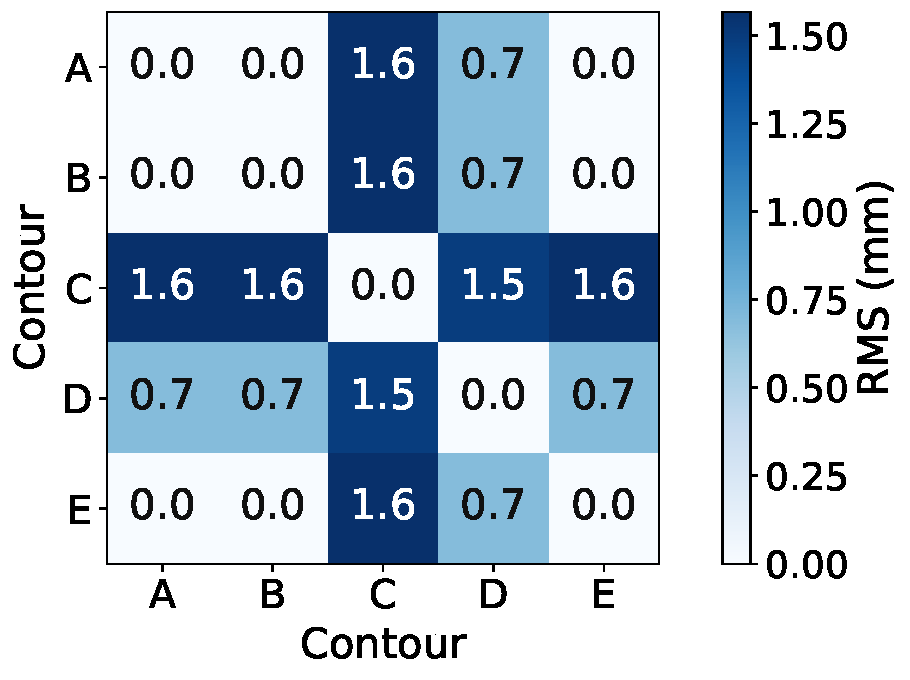
\includegraphics[width=.98\linewidth,height=.69\textheight,keepaspectratio]{presentation-figures/cohort-distances-panel-2.pdf}\end{frame}
\renewcommand{\notestarget}{notes.pdf\#note-cyclic-rigid-alignment}
\begin{frame}[t,fragile,label=slide-enumerate-the-starting-index]{Enumerate the starting index}
For each $k$, center the arrays, solve the proper Procrustes problem, and retain the smallest residual.\pause{} The identity choice guarantees $d_{rc}\le d_{\rm RMS}$.
\end{frame}
\renewcommand{\notestarget}{notes.pdf\#note-a-finite-cohort-and-its-comparison-rule}
\begin{frame}[t,fragile,label=slide-retained-geometric-differences]{Retained geometric differences}
Rigid copies and cyclic reindexings can have zero aligned discrepancy.\pause{} Size and local displacement remain nonzero because neither is removed by the allowed transformations.
\end{frame}
\renewcommand{\notestarget}{notes.pdf\#note-amplitude-and-neighbor-variation-penalties}
\begin{frame}[t,fragile,label=slide-equal-rms-does-not-imply-equal-displacement-pattern]{Equal RMS does not imply equal displacement pattern}
\[\frac1n\sum_j\|u_j\|^2\] measures amplitude but ignores how neighboring vectors vary.\pause{} Smooth and alternating fields can have the same value.
\end{frame}
\renewcommand{\notestarget}{notes.pdf\#note-amplitude-and-neighbor-variation-penalties}
\begin{frame}[t,fragile,label=slide-a-quadratic-neighbor-penalty]{A quadratic neighbor penalty}
\[E_\lambda(u)=\frac1n\sum_j\|u_j\|^2+\frac\lambda n\sum_j\|u_{j+1}-u_j\|^2.\]\pause{} $E_\lambda$ has units mm$^2$; $\lambda\ge0$ is dimensionless.
\end{frame}
\renewcommand{\notestarget}{notes.pdf\#note-amplitude-and-neighbor-variation-penalties}
\begin{frame}[t,fragile,label=slide-matrix-form-of-the-score]{Matrix form of the score}
\[E_\lambda(u)=\frac1n u^{\mathsf T}(I+\lambda D^{\mathsf T}D)u.\]\pause{} The identity term makes the matrix positive definite.
\end{frame}
\renewcommand{\notestarget}{notes.pdf\#note-fourier-interpretation-of-the-roughness-weight}
\begin{frame}[t,fragile,label=slide-scaling-and-constant-shifts]{Scaling and constant shifts}
\[E_\lambda(au)=a^2E_\lambda(u).\]\pause{} A constant displacement has zero neighbor penalty but nonzero amplitude cost.
\end{frame}
\renewcommand{\notestarget}{notes.pdf\#note-fourier-interpretation-of-the-roughness-weight}
\begin{frame}[label=slide-fourier-weights-of-roughness-panel-1]{Both RMS =\allowbreak{} 1 mm}
\centering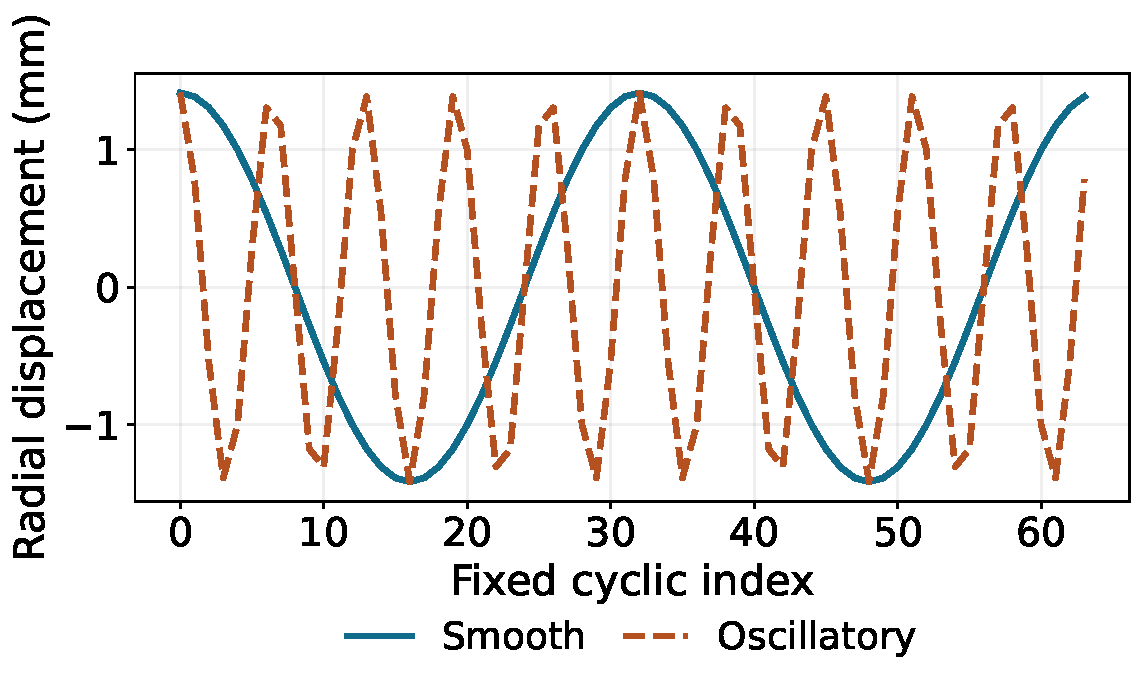
\includegraphics[width=.98\linewidth,height=.69\textheight,keepaspectratio]{presentation-figures/displacement-cost-panel-1.pdf}\end{frame}
\renewcommand{\notestarget}{notes.pdf\#note-fourier-interpretation-of-the-roughness-weight}
\begin{frame}[label=slide-fourier-weights-of-roughness-panel-2]{Same size, different roughness}
\centering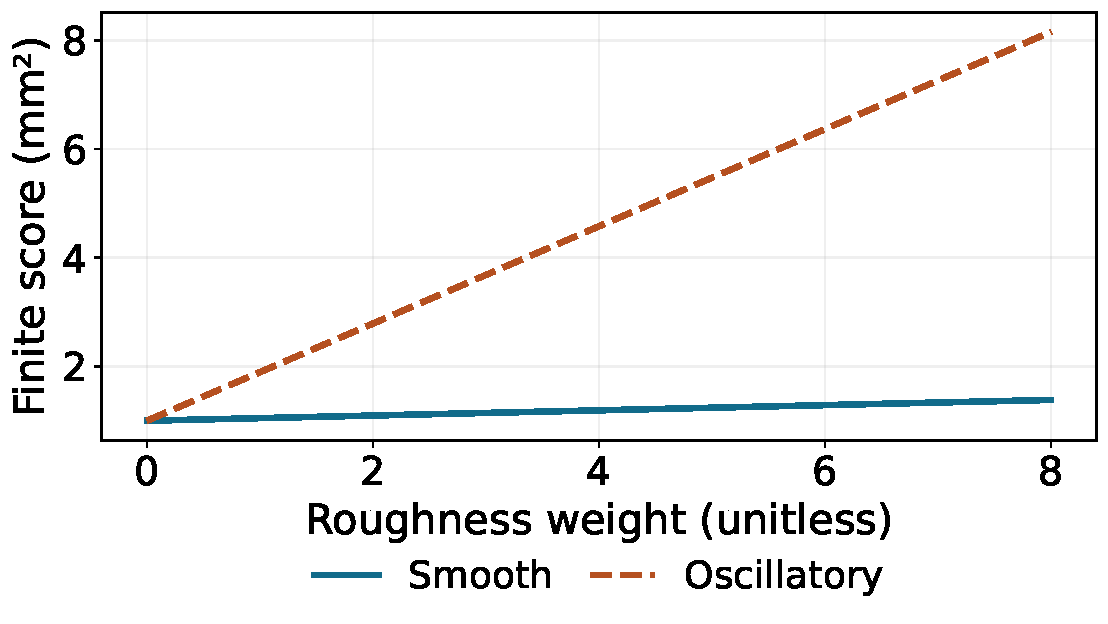
\includegraphics[width=.98\linewidth,height=.69\textheight,keepaspectratio]{presentation-figures/displacement-cost-panel-2.pdf}\end{frame}
\renewcommand{\notestarget}{notes.pdf\#note-fourier-interpretation-of-the-roughness-weight}
\begin{frame}[t,fragile,label=slide-fourier-weights-of-roughness]{Fourier weights of roughness}
\[E_\lambda=\sum_k[1+4\lambda\sin^2(\pi k/n)]\|\widehat u_k\|^2.\]\pause{} Higher-frequency displacement patterns receive greater penalty.
\end{frame}
\renewcommand{\notestarget}{notes.pdf\#note-fourier-interpretation-of-the-roughness-weight}
\begin{frame}[t,fragile,label=slide-the-grid-is-part-of-this-definition]{The grid is part of this definition}
The difference $u_{j+1}-u_j$ is not divided by arclength.\pause{} Changing sample density changes its interpretation as a derivative penalty.
\end{frame}
\renewcommand{\notestarget}{notes.pdf\#note-elastic-path-energy-and-varifold-endpoints}
\begin{frame}[t,fragile,label=slide-elastic-energy-along-a-path]{Elastic energy along a path}
\[\mathcal E(c)=\int_0^1G_{c(t)}(\dot c(t),\dot c(t))\,\mathrm dt.\]\pause{} A path metric measures deformation throughout a trajectory in shape space.
\end{frame}
\renewcommand{\notestarget}{notes.pdf\#note-elastic-path-energy-and-varifold-endpoints}
\begin{frame}[t,fragile,label=slide-endpoint-mismatch-is-a-separate-term]{Endpoint mismatch is a separate term}
\[\mathcal E(c)+\gamma\|\mu_{c(1)}-\mu_{target}\|_K^2.\]\pause{} The endpoint penalty promotes matching; it is not interchangeable with the path energy.
\end{frame}
\renewcommand{\notestarget}{notes.pdf\#note-elastic-path-energy-and-varifold-endpoints}
\begin{frame}[t,fragile,label=slide-nonoriented-geometric-comparison]{Nonoriented geometric comparison}
Positions, geometric weights and tangent or normal directions define an endpoint representation.\pause{} Squared directional dot products can identify opposite orientations. Kernel scale controls spatial sensitivity.
\end{frame}
\renewcommand{\notestarget}{notes.pdf\#note-invariant-comparisons-and-scientific-interpretation}
\begin{frame}[t,fragile,label=slide-the-implemented-and-contextual-calculations]{The implemented and contextual calculations}
The companion computes finite cyclic alignment and a quadratic displacement score.\pause{} Elastic surface paths and varifold registration remain research context, with additional geometry, optimization and numerical requirements.
\end{frame}
\end{document}
